\begin{figure}
\centering
\subfloat[\label{fig:fractionabundancescellcount}]{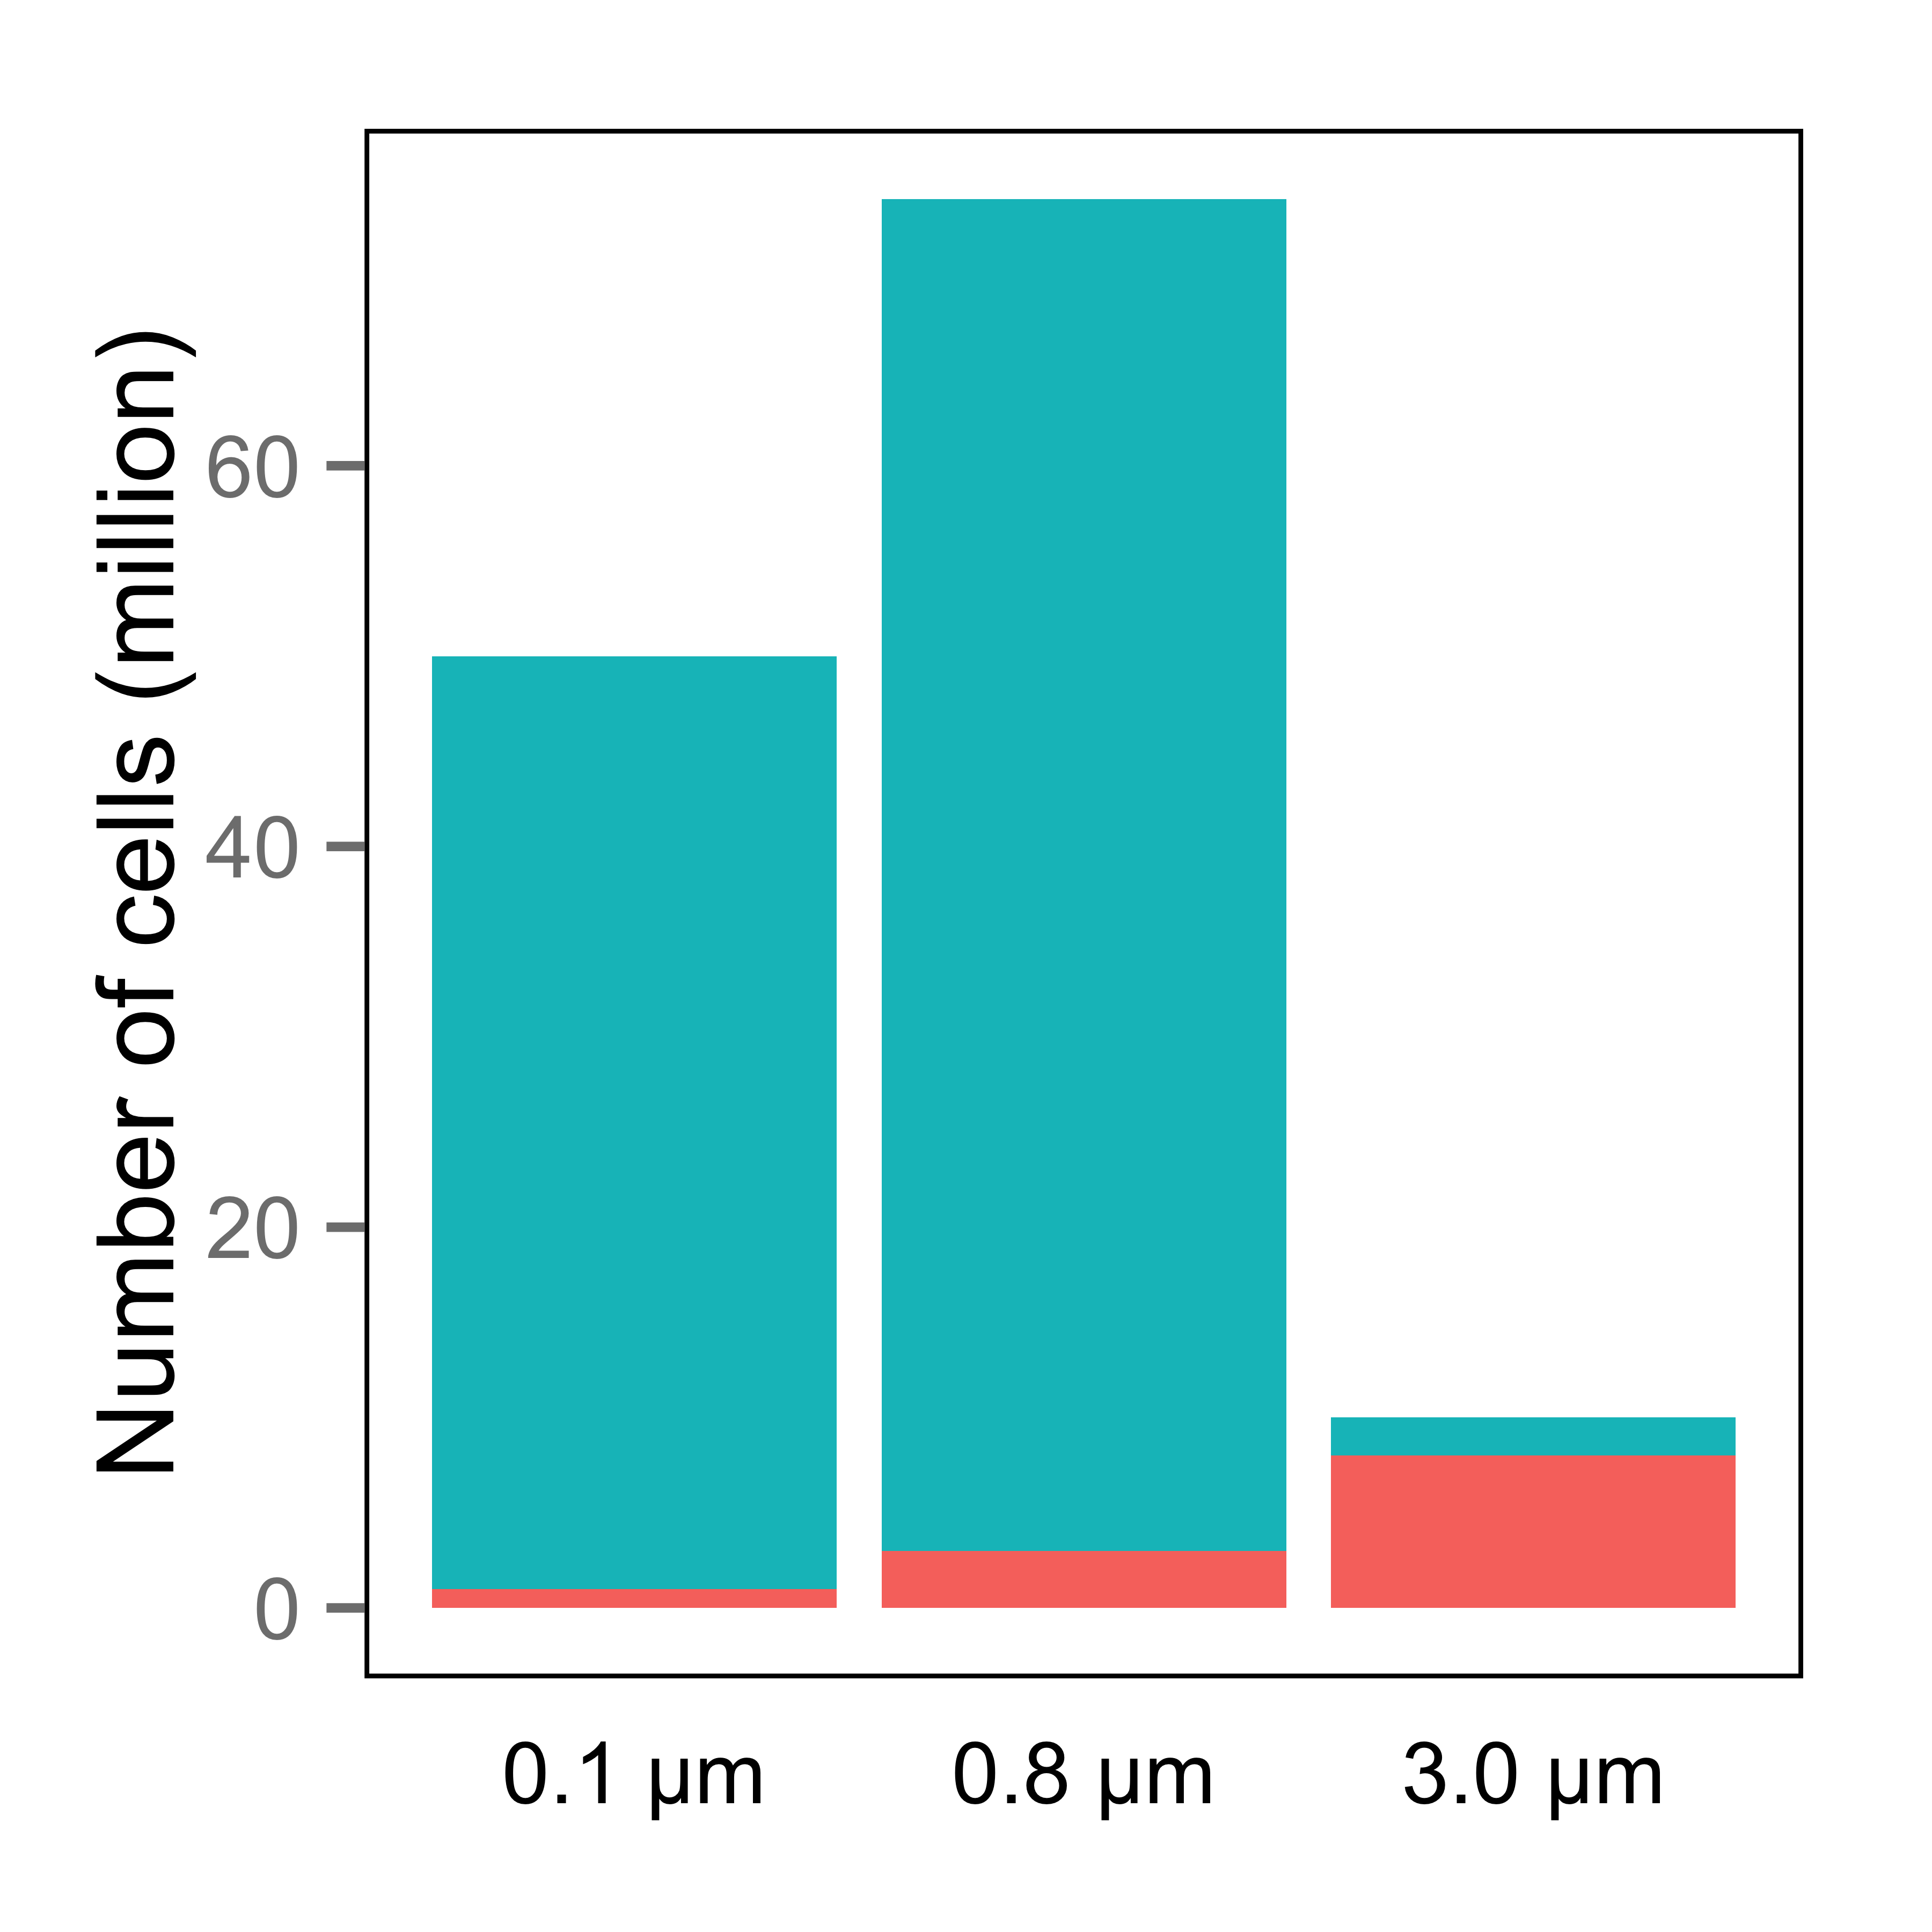
\includegraphics[scale=0.04]{../polarfront/fractionabundances1.png}}
\quad
\subfloat[\label{fig:fractionabundancesrelative}]{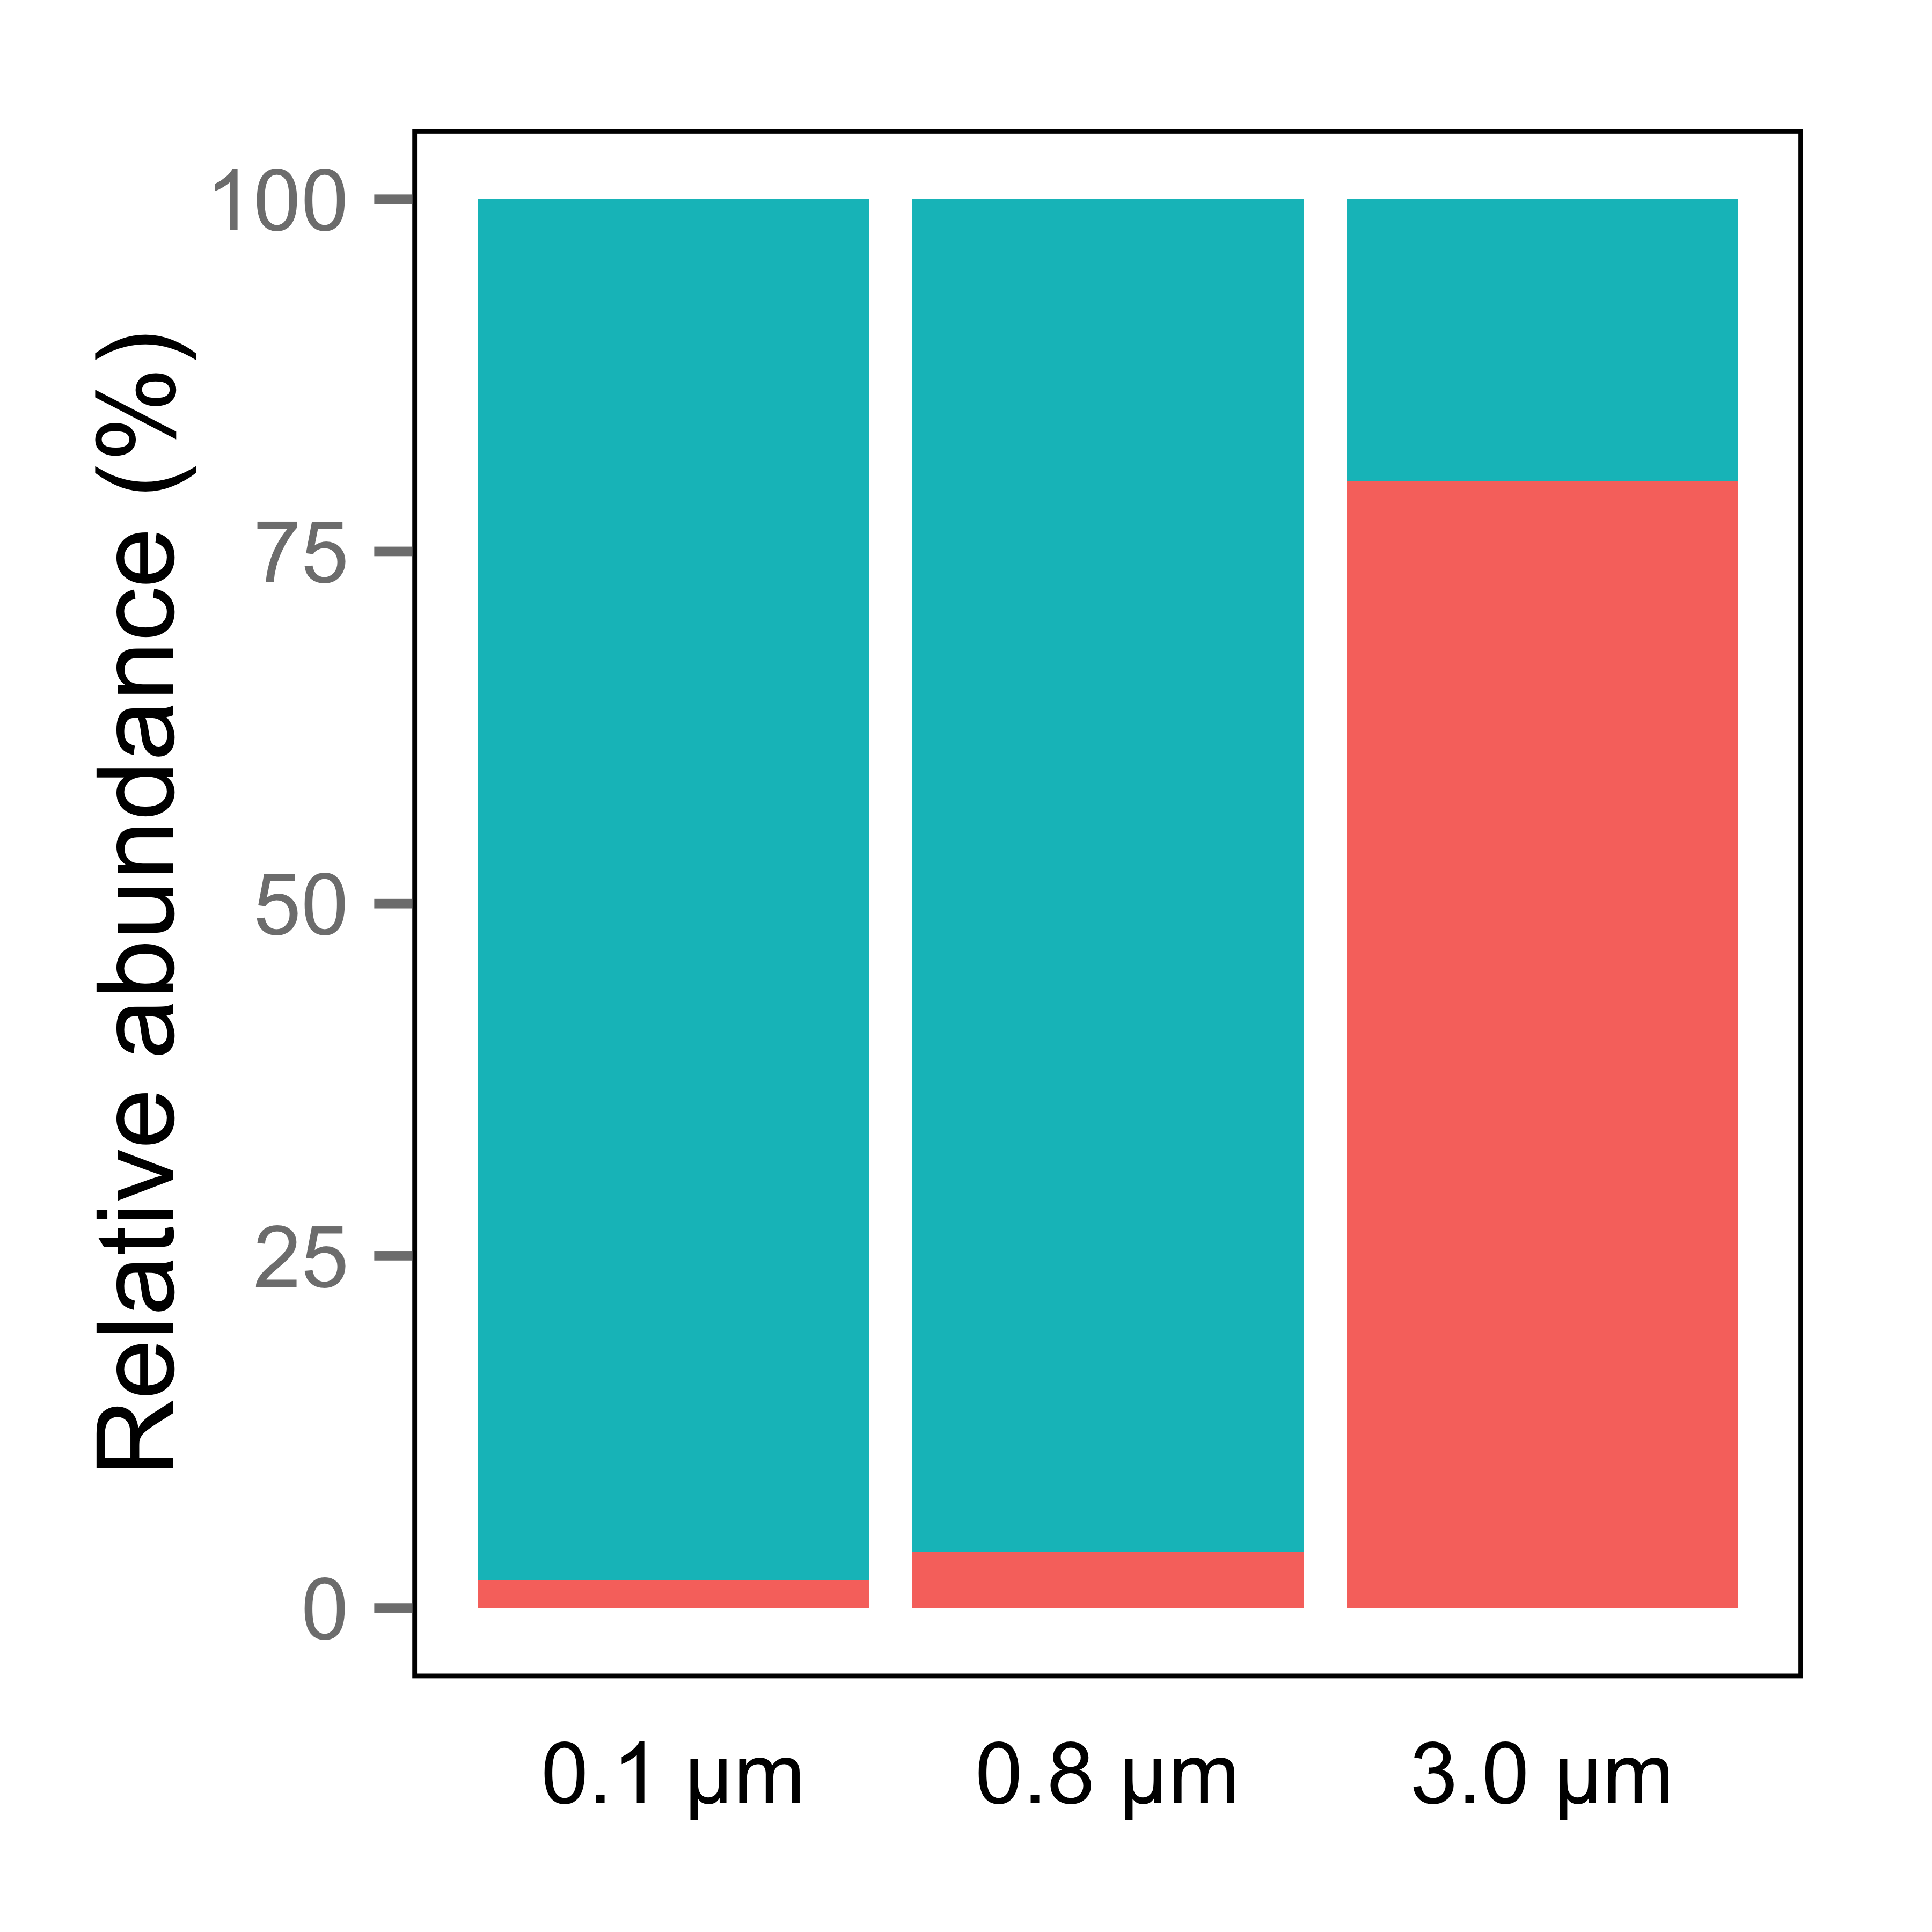
\includegraphics[scale=0.04]{../polarfront/fractionabundances2.png}}
\quad
\subfloat[\label{fig:fractionabundancescombined}]{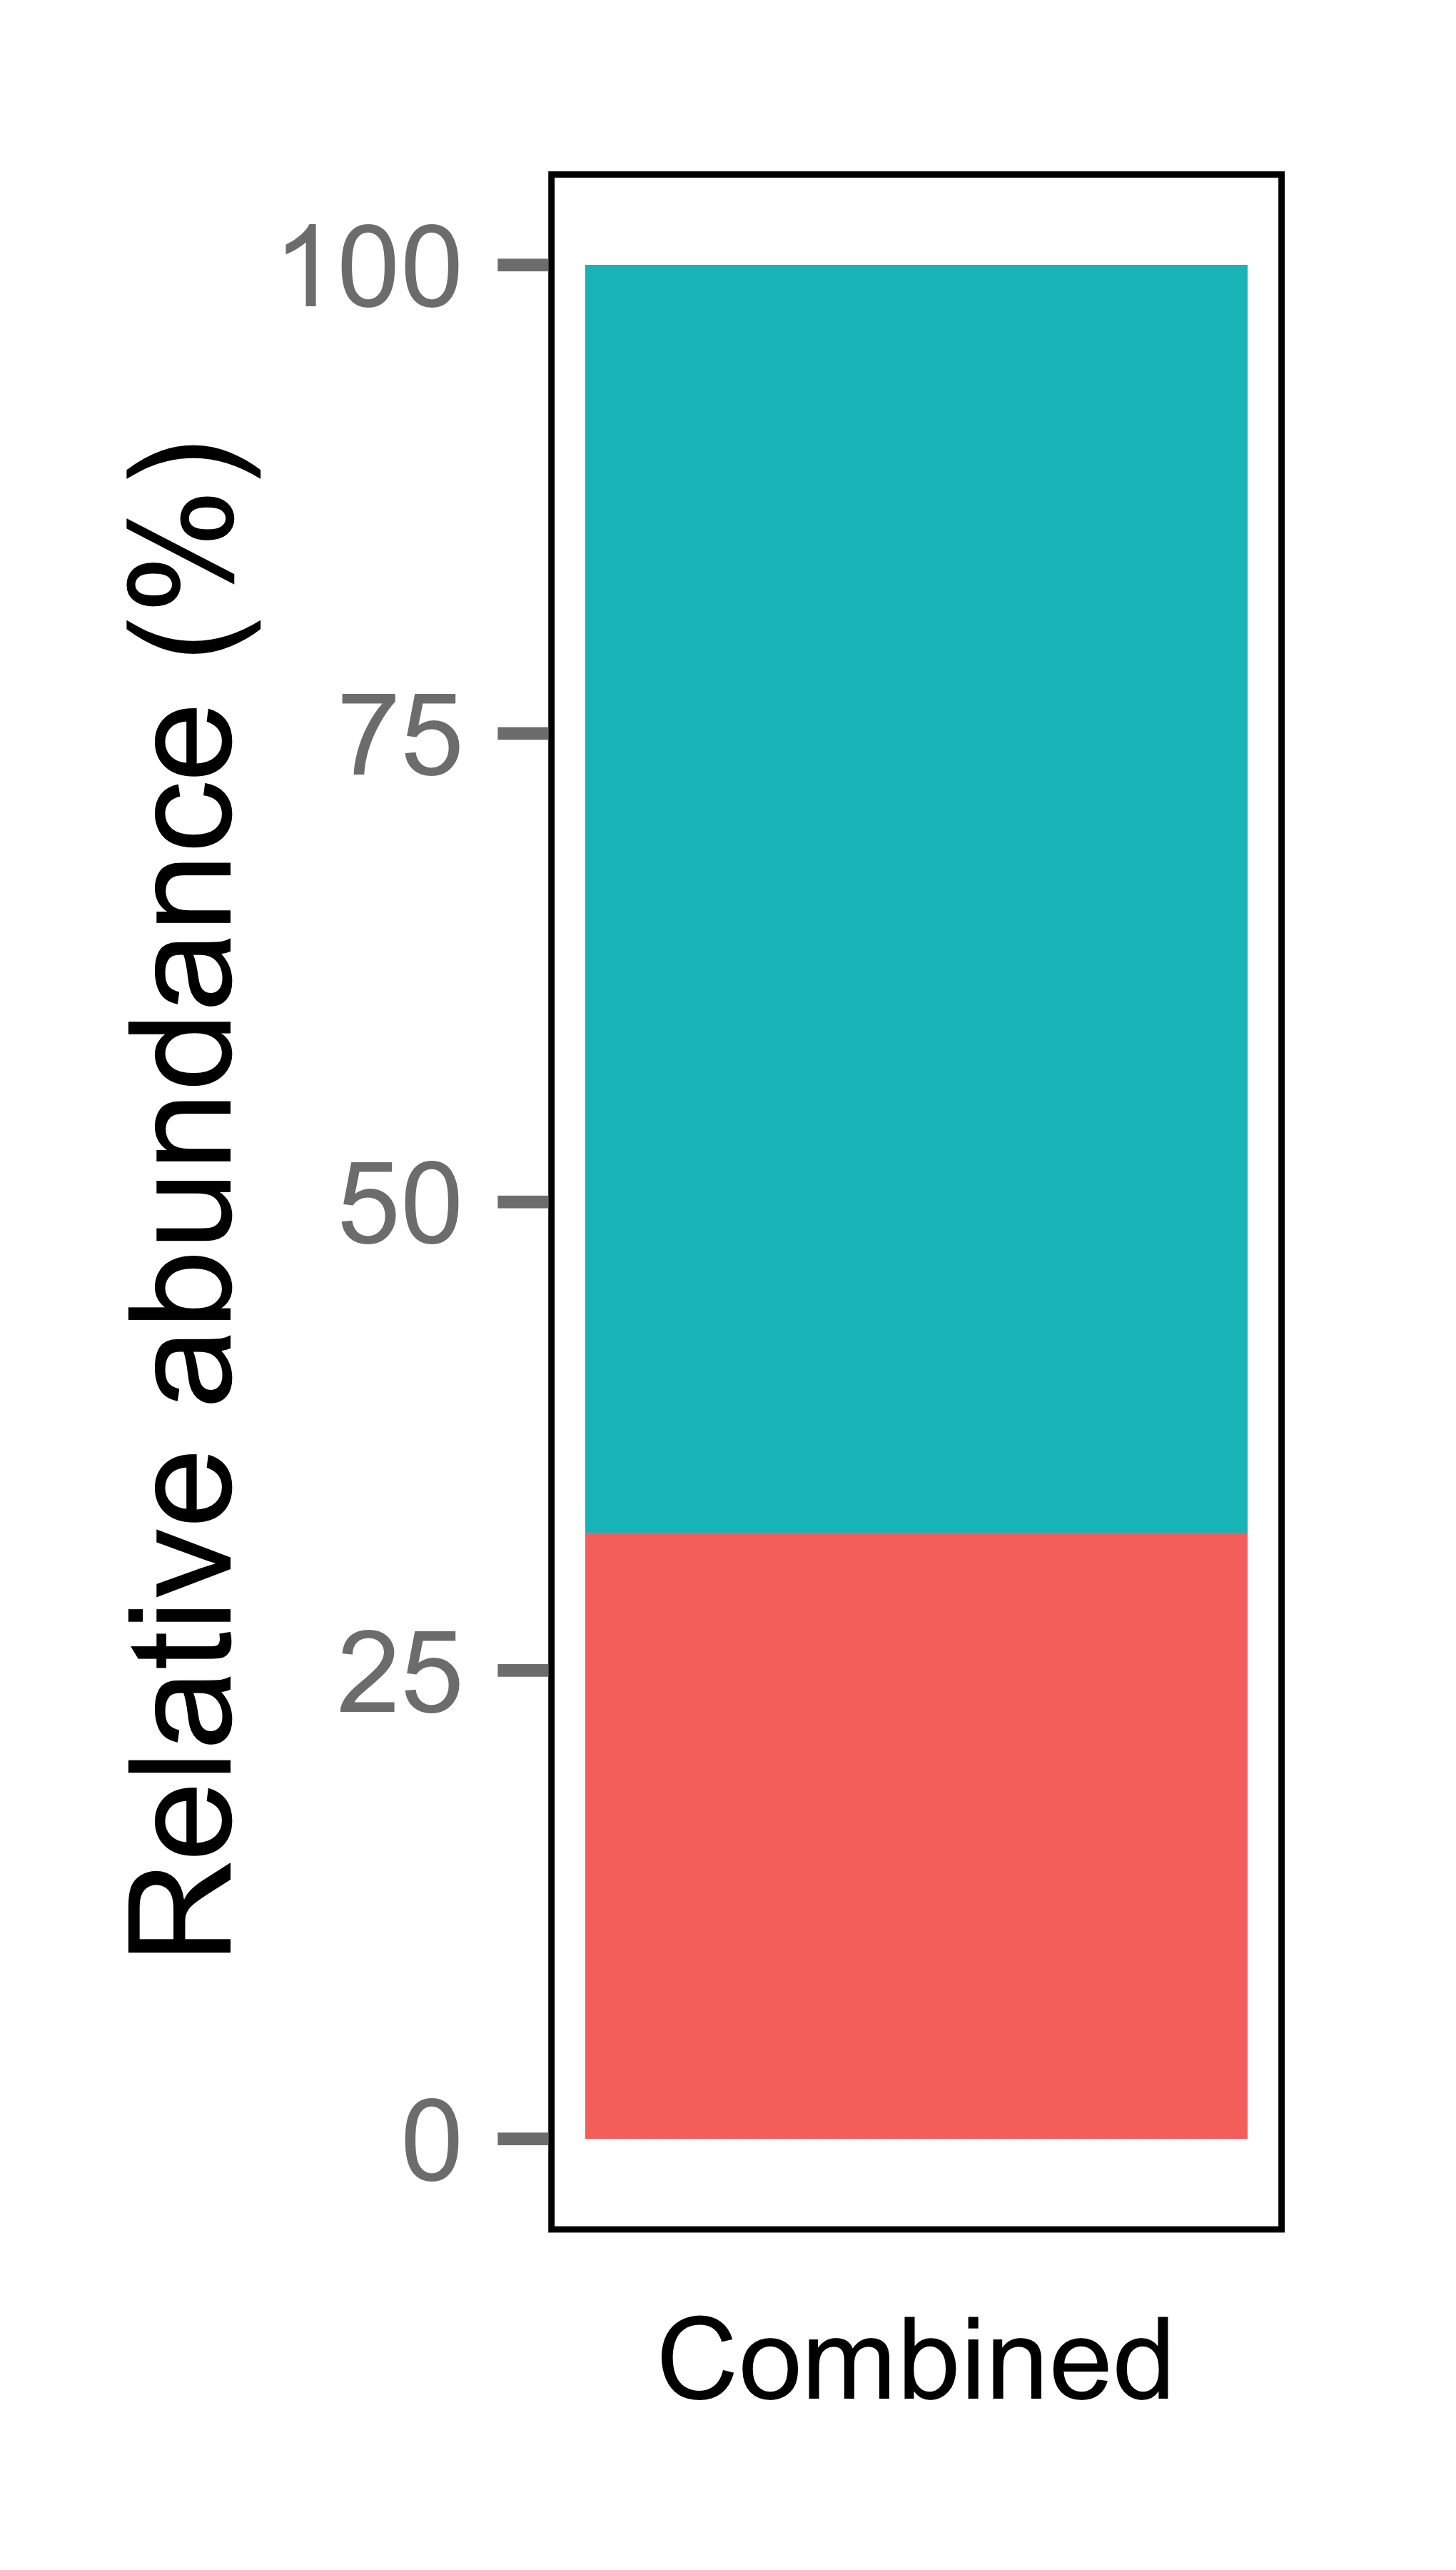
\includegraphics[scale=0.04]{../polarfront/fractionabundances3.png}}
\caption[Summing relative abundances across size fractions]{An example of distortion introduced by summing OTU relative abundances across size fractions. The red OTU composes only 15\% of the total number of cells captured (a). However, it is enriched (80\%) in the 3.0 \micron{} fraction (b). If the relative abundances are simply summed, the red OTU appears to compose 30\% of the community, twice the correct value (c). Without cell counts for each fraction, relative abundances cannot be summed between the fractions.}
\label{fig:fractionabundances}
\end{figure}
